% =============================================================================
% The CGAL Developers' Manual
% Chapter: Specification Documentation
% -----------------------------------------------------------------------------
% file   : specification.tex
% authors: Susan Hert <hert@mpi-sb.mpg.de>
% -----------------------------------------------------------------------------
% $Id$
% $Date$
% =============================================================================

\newcommand{\macroitem}[1]{%
    \item[{\normalfont \textbf{\texttt{\ccBackslash #1}}%
    }]%
    \index{#1@{\tt\protect\ccBackslash #1}}~\par
}
\newcommand{\macroitemX}[2]{%
    \item[{\normalfont \textbf{\texttt{\ccBackslash #1}}%
      \textbf{\texttt{\ccOpenBrace}}\emph{#2\/}\textbf{\texttt{\ccCloseBrace}}%
    }]%
    \index{#1@{\tt\protect\ccBackslash #1}}~\par
}
\newcommand{\macroitemXX}[3]{%
    \item[{\normalfont \textbf{\texttt{\ccBackslash #1}}%
      \textbf{\texttt{\ccOpenBrace}}\emph{#2\/}\textbf{\texttt{\ccCloseBrace}}%
      \textbf{\texttt{\ccOpenBrace}}\emph{#3\/}\textbf{\texttt{\ccCloseBrace}}%
    }]%
    \index{#1@{\tt\protect\ccBackslash #1}}~\par
}
\newcommand{\macroitemXXX}[4]{%
    \item[{\normalfont \textbf{\texttt{\ccBackslash #1}}%
      \textbf{\texttt{\ccOpenBrace}}\emph{#2\/}\textbf{\texttt{\ccCloseBrace}}%
      \textbf{\texttt{\ccOpenBrace}}\emph{#3\/}\textbf{\texttt{\ccCloseBrace}}%
      \textbf{\texttt{\ccOpenBrace}}\emph{#4\/}\textbf{\texttt{\ccCloseBrace}}%
    }]%
    \index{#1@{\tt\protect\ccBackslash #1}}~\par
}


\chapter{Specification Documentation\label{chap:specification}}

\ccChapterRelease{Chapter Version: 2.0}
\ccChapterAuthor{Susan Hert ({\tt hert@mpi-sb.mpg.de})\\
                 Lutz Kettner ({\tt kettner@mpi-sb.mpg.de}) }
\ccIndexMainItemBegin{manuals}


\begin{quote}
There are two ways of constructing a software design.  One way is to make
it so simple that there are obviously no deficiencies.  And the other way
is to make it so complicated that there are no obvious deficiencies.

\hspace*{\fill}{\em C. A. R. Hoare}
\end{quote}

\cgal\ is physically structured into
packages\ccIndexMainItem{package}, which is reflected in the SVN
repository structure.  Generally, each
package in the library will contribute some chapters to the manuals,
some might only contribute a section to some larger chapter.

Generally, a manual is created for the whole \cgal\ library.
However, manuals can be created for individual packages,
mostly for editing and reviewing, and also only reasonably if the
package contributes a whole chapter.

The official \cgal\
\ccAnchor{http://www.cgal.org/Manual/}{documentation}
is currently divided into three separate manuals:
\begin{itemize}
   \item User and Reference Manual
   \item Installation Guide
   \item Developers Manual
\end{itemize}
Not surprisingly, the Installation Guide describes how to install \cgal
\ccIndexMainItem{installation}. It is also integrated as a chapter in the
User and Reference Manual.
% The developers manual may be replaced by the wiki rather soon.

Documentation of new packages and features will likely be included in
the User and Reference Manual.  It is further
subdivided into several parts representing the overall thematic structure
of \cgal, each part containing chapters, each chapter having a user
and a reference manual.
Sections~\ref{sec:users_manual} and~\ref{sec:ref_manual} below
describe the contents of these two manuals.

The manuals are produced from \LaTeX\ input files in PDF and
HTML formats. We provide a set of style files with numerous commands
that are used to format the manuals in a (more or less) uniform fashion.
The conversion from \LaTeX\ input to HTML output is done with
our own \texttt{latex\_to\_html} converter program that in particular
understands our manual style files.
Section~\ref{sec:files_required} describes how to organize your
documentation files and what is required for submitting documentations.
Section~\ref{sec:manual_tools} provides the basic information about
these tools and style files that you will need to produce
the documentation for your package.
Sections~\ref{sec:ref_manual} and~\ref{sec:users_manual} describe the
contents and the macros provided in our style files for the Users'
Manual and the Reference Manual, respectively.
Sections~\ref{sec:doc_figures} and~\ref{sec:indexing} give information
about including figures in your documentation and inserting indexing
commands, respectively.
Section~\ref{sec:doc_test_suite} describes the manual test suite run
for each internal release of the library.
Section~\ref{sec:common_problems} discusses common problems and
solutions.
Section~\ref{sec:spell_checker} documents the use of a spell checking system
and custom dictionary for \cgal\ manuals.
Section~\ref{sec:specification_req_and_rec} concludes with the
requirements and recommendations for the specification documentation.

% =============================================================================
\section{File and directory organization\label{sec:files_required}}
\ccIndexSubitemBegin{manuals}{source files}
\ccIndexSubitemBegin{source files}{documentation}

We start with the organization of the documentation of a package.
After that, we describe the organization of a module documentation.

Generally, each package in the library will have its own chapter in
both the reference manual and the users' manual%
\ccIndexMainItem{users' manual}%
\ccIndexMainItem{reference manual}, some might only contribute a
section to some larger chapter. So, in principle, the documentation of
a package starts with the \verb|\ccUserChapter| or \verb|\ccRefChapter|
commands. Note, that each chapter, in particular the \verb|\ccUserchapter|
command, needs to be in a different file. A wrapper file may then include
all chapters.

The \texttt{Polyhedron} package can serve as an example for the manual
organization.

\ccIndexSubitem{directory structure}{for documentation}
It is required that the documentation submitted with a package be organized
according to a specific directory structure. In summary, all
{\tt .tex} source files and corresponding figures are kept in a
\texttt{doc\_tex} subdirectory of the package. The following rules
describe the details:

\begin{itemize}
   \item The programs creating the manuals, i.e., \texttt{latex},
         \texttt{pdflatex} etc.,
         are called in the \texttt{doc\_tex} directory. Since
         \texttt{latex}, and consequently \texttt{latex\_to\_html}
         too, do not maintain a current working directory, all
         filenames, such as in include statements, figures, etc., must
         be given relative to this \texttt{doc\_tex} directory.
   \item The input search paths of \texttt{latex} and
         \texttt{latex\_to\_html} will be enriched with the paths for
         example and demo programs, such that they can be referenced
         starting from their package subdirectory name, e.g.,
         \verb|\ccIncludeExampleCode{Polyhedron/polyhedron_prog_simple.cpp}|.
   \item The {\tt .tex} files for the users' manual%
         \ccIndexSubitem{users' manual}{directory} should be placed in a
         directory \verb|doc_tex/|$<${\em Package}$>$\verb|/|%
         \index{doc_tex directory@{\tt doc\_tex} directory}. Among
         them, the file {\tt main.tex}\ccIndexMainItem{\tt main.tex}%
         \ccIndexSubitem{users' manual}{\tt main.tex}
         must exist that inputs all other users'
         manual source files using the \verb|\input| command (NOT the
         \verb|\include| command).%
         \index{input@$\backslash${\tt input}!vs. include@vs.
           $\backslash${\tt include}}.
         \ccIndexSubitem{manuals}{new style}%
         \ccIndexMainItem{reference manual}

   \item The {\tt .tex} files for the reference manual should be placed in the
         directory \verb|doc_tex/|$<${\em Package}$>$\verb|_ref/|.
         \ccIndexSubitem{directory structure}{for reference manual}%
         \ccIndexSubitem{reference manual}{directory}%
         \index{ref directory@{\tt \_ref} directory}%
         Also among them, the file {\tt main.tex} must exist that
         inputs all other reference manual source files.
         For the purposes of the \LaTeX -to-HTML converter, each item
         documented in the reference manual should be put in its own file.
         \ccIndexSubitem{reference manual}{files}
         (The script \ccAnchor{#cc_ref_wizard}{{\tt cc\_ref\_wizard}} can help
          in creating these files.)
         The script \ccAnchor{#cc_make_ref_pages}{{\tt cc\_make\_ref\_pages}}
         will create a {\tt main.tex}%
         \ccIndexSubsubitem{reference manual}{\tt main.tex}{creating}
         file given the name of the directory that contains the separate files
         for each
         reference manual item.  The items will be input in alphabetical order,
         with a file {\tt intro.tex}\ccIndexMainItem{\tt intro.tex}, if it
         exists, included first.  The {\tt intro.tex} file should
         start with the \verb|\ccRefChapter| command, then the
         \verb|\ccChapterAuthor| command. It should also
         contain a short introductory section, give an overview of the
         reference pages contained in this chapter, and mention
         optionally with a non-numbered section labeled \textbf{Assertions}
         the string used in the package-specific assertion macros.
\end{itemize}

This is all that is needed for a package manual and the
\texttt{cgal\_manual} program mentioned in
Section~\ref{subsec:cgal_manual_program} will create the necessary
wrapper file automatically on the fly to create PDF, or
HTML manuals for an individual package.

For modules (collections of packages, note: maybe an outdated idea),
an additional wrapper file is needed.
The following rules describe the details, and
Section~\ref{subsec:wrapper_module_manual} lists an example wrapper file:

\begin{itemize}
   \item To be detected automatically by the tools in
         Section~\ref{sec:manual_tools} the wrapper filename must
         match the pattern {\tt *\_manual.tex}.
   \item Wrapper files must be placed in the \texttt{doc\_tex}
         subdirectory. Wrapper files that do not have a good package
         where they would belong to can be kept in the \texttt{Manual}
         SVN package, for example, \texttt{cgal\_manual.tex}
         containing the manual for whole \cgal.
\end{itemize}

\ccIndexSubitemEnd{source files}{documentation}
\ccIndexSubitemEnd{manuals}{source files}


% =============================================================================
\section{The manual tools\label{sec:manual_tools}}
\ccModifierCrossRefOff
\ccIndexSubitemBegin{tools}{manual}

As a package author, it suffices to learn from this section that you
need to install two SVN packages, how to use the \texttt{cgal\_manual}
program, and what style files are available in the automatically
generated wrapper for packages. Occasionally, you might need to add a
new entry in the globally maintained Bib\TeX\ file.

For module authors, we list an example wrapper file and document the
commands available in particular for wrapper files and for handling
dependencies between packages. The example wrapper file might also be
helpful for package authors to understand the context in which the
package chapter is formatted.

All programs, style files, and other supporting files for the creation
of the manuals are contained in two SVN packages:
\ccIndexSubsubitemDef{tools}{manual}{SVN package}
\index{SVN server!Manual_tools package@\texttt{Manual\_tools} package}
\ccIndexSubitemDef{manual}{SVN package}
\index{SVN server!Manual package@\texttt{Manual} package}

\begin{description}
    \item[\textbf{Manual\_tools}]
        contains the style files for \CC\ manual page formatting
        and the \LaTeX\ to HTML converter program. These style files
        and the converter can be used independently from \cgal.
        Stable snapshots are also supposed to be released at
        \path|http://www.cgal.org/Members/Manual_tools/| (but it has not
        been done for a long time).
    \item[\textbf{Manual}]
        contains the \cgal\ specific \LaTeX\ wrapper files with the
        customization for the \cgal\ manuals and a top-level driver
        script to run \LaTeX\ and the \texttt{latex\_to\_html}
        converter consistently in the manual file structure of \cgal\
        manuals. It contains also the additional auxiliary files for
        creating the \cgal\ manuals that are not particular to
        individual packages. These are figures like the \cgal\ logo or
        the bibliography file \texttt{doc\_tex/Manual/cgal\_manual.bib}
        for Bib\TeX.
\end{description}

In a nutshell, it is mandatory to install the \texttt{Manual\_tools}
package properly on your system. From the \texttt{Manual} package one
needs only the program \texttt{Manual/developer\_scripts/cgal\_manual}
in the execution path and the package itself should be placed
side-by-side with your own package(s) that you develop (the
\texttt{cgal\_manual} script finds then automatically the other files
in the \texttt{Manual} package). Side-by-side means that the package
directory \texttt{Manual} is in the same directory as the package
directory \texttt{Package} that you develop.


% -----------------------------------
\subsection{Program \texttt{cgal\_manual} in the \texttt{Manual} package}
\label{subsec:cgal_manual_program}

The \texttt{cgal\_manual} program is a \texttt{bash} script residing
in the \texttt{developer\_scripts/} directory. It is called in the
\texttt{doc\_tex/} directory of a \cgal\ package or of an internal
release.

This script is the driver program for creating \cgal\ manuals.  It
makes use of PDF\LaTeX, Bib\TeX, \texttt{makeindex},
\texttt{latex\_to\_html}, and other tools to create the
PDF and HTML manuals for individual \emph{SVN Packages} as well as
custom \emph{Modules} and its \emph{Sub-Modules}. It encodes the conventions
of how \cgal\ manuals are organized and how the general purpose tools need
to be called to create the manuals. We specify these conventions here in the
developers manual. Note that a brief documentation is also kept in the
script itself, these documentations need to be kept synchronized!

\begin{description}
  \item[SVN Package]~

     Development unit in \cgal\ hosted on our SVN server. A package has a
     fixed directory structure. Let's assume the package is
     called \texttt{Geom}, then the documentation must reside in a directory
     \texttt{doc\_tex/} within the package \texttt{Geom}. Here,
     individual subdirectories, typically \texttt{Geom/} and
     \texttt{Geom\_ref/}, contain the users' and the reference
     manual respectively. The individual subdirectories contain a
     \texttt{main.tex} file that contains the manual chapter, possibly
     several and possibly using several other input files, but all
     included with relative paths from the \texttt{doc\_tex/}
     directory, where the tools and this script will run.

     In general, all individual subdirectories that contain a
     \texttt{main.tex} file are processed. If they exist in pairs, we
     assume that \texttt{doc\_tex/*/main.tex} and
     \texttt{doc\_tex/*\_ref/main.tex} are corresponding users' and
     reference manual entries in the table of contents.

     The \texttt{main.tex} files are not stand-alone \LaTeX\ files. They are
     chapters, i.e., do not contain \verb|\begin{document}| commands
     etc. This script provides the necessary \LaTeX\ wrapper file.

   \item[Modules \emph{(advanced feature)}]~

     Presentation unit of modularity towards the user, assembled from
     SVN Packages. For a module of name \texttt{Algo} it is assumed
     that in the \texttt{doc\_tex/} directory  the necessary \LaTeX\
     driver file \texttt{Algo.tex} exists.
     This driver is a complete \LaTeX\ file including the
     \verb|\begin{document}| command and such. It includes the various
     chapters from the packages.

   \item[Sub-Modules \emph{(advanced feature)}]~

     Another presentation unit on top of modules. A sub-module only contains
     a subset of the packages in a module. The numbering of pages,
     chapters, equations et cetera is inherited from the module, while the
     table of context and the index is shrink-wrapped to the sub-module.

     Generally, for some module \texttt{m.tex}, a sub-module \texttt{sub} is
     defined in a file \texttt{m\_\_sub.only.tex} that contains \LaTeX\
     commands to be executed before the document starts. The most obvious
     command therein is probably \texttt{$\backslash$includeonly}. Note: packages split
     into user manual and reference manual need two entries in the
     \texttt{\\includeonly} command. Sub-modules have to adhere to the
     filenaming scheme from above, in order to be found by the
     \texttt{cgal\_manual} script. There can be multiple sub-modules for each
     module. Sub-modules of sub-modules are not supported.

     For example, consider a module stored in \texttt{cgal\_manual.tex}. A
     sub-module \texttt{Geom} should be built, restricting the module to user
     and reference manual of the package \texttt{Geom}. It could be stored in
     a file called \texttt{cgal\_manual\_\_Geom.only.tex}, only containing the
     \LaTeX\ command
     \texttt{$\backslash$includeonly\{Geom/main,Geom\_ref/main\}}.

     When building a module with the \texttt{cgal\_manual} script, the
     default is to produce no sub-modules of it. The desired sub-modules
     can be specified by \texttt{-sub-modules=mod1,mod2..} where sub-modules
     are given as a comma-separated list. Only the sub-module name has to be
     given, not the filename under which it is stored. A special sub-module
     is \texttt{all}, which matches all sub-modules present in the current
     directory.
\end{description}

 This script can create individual package documentation given the name of
 the individual subdirectories in \texttt{doc\_tex/}. It creates module
 documentations given the name of the module \LaTeX\ driver file.

 The default is to create package manuals for all \texttt{*/main.tex} files,
 where \texttt{*/main.tex} and corresponding \texttt{*\_ref/main.tex}
 are kept in one manual, and to create manuals for all
 \texttt{*\_[Mm]anual.tex}, which are representing modules.

 This script can be used in three different environments of \cgal\ sources.
 It decides automatically in which situation it is and adapts the necessary
 search paths for style files and bibliographies.

\begin{enumerate}
  \item \textbf{\cgal\ Internal Release:}
     The style and bibliography files are relative from the
     \texttt{doc\_tex} directory  in the subdirectory
     \texttt{Manual/}.

  \item \textbf{Individual \cgal\ Packages + \cgal\ Package \texttt{Manual}:}
     The style and bibliography files are  relative from the
     \texttt{doc\_tex} directory reachable with the path
     \texttt{../../Manual/doc\_tex/Manual/}.

   \item \textbf{All other environments:}
     The style and bibliography files need to be installed properly
     from the SVN package \texttt{Manual}, such that the tools can
     find them, for example, through the search paths defined in the
     environment variables  \texttt{TEXINPUTS}, \texttt{BIBINPUTS},
     and \texttt{LATEX\_CONV\_INPUTS}. The program checks if the files
     are actually in the search paths and issues an error message otherwise.
\end{enumerate}

This script properly adds entries in \texttt{TEXINPUTS},
\texttt{BIBINPUTS}, and \texttt{LATEX\_CONV\_INPUTS} so that bib and
style files are found. It also adds \texttt{../examples:../demo} to
these paths so that example source codes are properly found.

The result of run of \texttt{cgal\_manual} are the specified manuals
in the corresponding \texttt{../doc\_ps}, \texttt{../doc\_pdf}, and
\texttt{../doc\_html} directories. A logfile with suffix
\texttt{.cgallog} is created with a logfile summary from the
individual logfiles \texttt{.log}, \texttt{.blg}, \texttt{.ilg},
\texttt{.pdflg}, and \texttt{.hlg}. The logfiles are kept in case of
warnings and error messages.

The screen output reports the progress and result status of each
module (abbreviated as \texttt{Mod}) and package (abbreviated as
\texttt{Pck}) for each manual type, i.e., PDF and HTML.

This script also serves for the test-suite. It can be configured to
create the test-suite result tables also at your local configuration
(and without sending the email notification to cgal-develop ;-).
The default settings are encoded and documented at the beginning of
the script in a clearly marked region. For individual customizations,
the script reads the individual resource file
\verb|${HOME}/.cgalmanualrc| after the default initialization.

When the \texttt{-testsuite} option is used the script will copy all
the manuals and logfiles to
\verb|${TestSuiteResultPath}/CGAL-${CgalVersion}/| and creates an HTML
summary page \texttt{index.html} in that subdirectory. The latest
result is also always accessible at
\verb|${TestSuiteResultPath}/LAST/index.html|.  Furthermore, the
script will cleanup old results. For the most recent number
\verb|${TestSuiteFullHistory}| of test suites the full results
including the manuals are kept. Older test suites will have their
manuals deleted to save space. In total only
\verb|${TestSuiteHistory}| many test suites are kept.  The history of
test suites is managed in a shift register like fashion using files of
defined names \texttt{History.<i>} that contain the name of the $i$-th
test suite subdirectory. The 1st is the most recent test suite and
corresponds to the \texttt{LAST} directory.  If the test suite is
repeated for the same internal release number, the new results will
overwrite the old results.


\begin{alltt}
\textbf{Usage: cgal\_manual [<options>] [<module-files...>] [<package-dirs...>]}
\textbf{Options:}
    \textbf{-pdf      }          PDF manuals.
    \textbf{-html     }          HTML manuals (incl. a LaTeX run).
    \textbf{-wrapper  }          creates the LaTeX wrapper files only.
    \textbf{-testsuite}          runs testsuite, installs results and sends email. Use
    \textbf{          }          only after reading the config section of this script.
    \textbf{-h        }          help.
    \textbf{-V        }          version.
    \textbf{-v        }          verbose: repeats logfiles on stderr.
    \textbf{-k        }          keep logfiles (default: delete after a clean run).
    \textbf{-n        }          no logfile: delete logfiles always.
    \textbf{-s        }          create a summary logfile .sum .
    \textbf{-quiet    }          no progress messages.
    \textbf{-realquiet}          suppresses also error messages.

    \textbf{-cmdlog   }          create a logfile "cmd_log" containing all commands
                          that were issued during execution

    \textbf{-sub-modules=mod1,mod2...}
                          build specified sub-modules, given as a comma-
                          separated list.
\end{alltt}


% -----------------------------------
\subsection{SVN package \texttt{Manual\_tools}}

The SVN package \texttt{Manual\_tools} keeps all files in the
subdirectory called \texttt{Manual\_tools}, which itself has
the following subdirectories:

\begin{description}
   \item[{\bf\tt doc\_tex/}] -- directory containing the documentation for
        the style files and the converter program
   \item[{\bf\tt example/}] -- directory containing example documentation
   \item[{\bf\tt scripts/}] -- directory containing various support scripts
   \item[{\bf\tt src/}] -- directory containing the style files and program
        source code for the \LaTeX\ to HTML converter
   \item[{\bf\tt sty/}] -- directory containing the \LaTeX\ style files
        used for formatting the manual.
\end{description}

There are also \texttt{README} and \texttt{CHANGES} files provided for
information. It is mandatory to install this package properly on your
system following the description in the \texttt{INSTALLATION} file. Linux
and Sun Solaris are supported platforms. Cygwin on Windows is also
supported as soon as a proper LaTeX distribution is installed, and
found in the PATH.

\subsection{Style files in the \texttt{Manual\_tools} package}
\label{subsec:manual_tools_style_files}
\ccIndexSubsubitem{tools}{manual}{style files}

The manuals are written with macros provided in the following style
files provided in the \texttt{Manual\_tools} package. When properly
installed, these style files are in the search paths of \LaTeX\ and
\texttt{latex\_to\_html}. The most prominent macros are introduced in
this chapter. For the full documentation please see to the files with
corresponding names in the \texttt{Manual\_tools/doc}
directory\ccIndexSubsubitem{tools}{manual}{documentation}.

\begin{itemize}
   \item {\tt cc\_manual.sty}\ccIndexMainItem[c]{\tt cc_manual.sty}
       provides the commands to structure \CC\ reference manuals
       and to format \CC\ declarations nicely.
   \item {\tt cc\_manual\_index.sty}\ccIndexMainItem[c]{\tt
       cc_manual_index.sty} provides the commands for creating an
       index.
   \item {\tt latex\_converter.sty}\ccIndexMainItem[c]{\tt latex_converter.sty}
       provides commands useful for the conversion to HTML.
\end{itemize}


% -----------------------------------
\subsection{Programs in the \texttt{Manual\_tools} package}
\label{subsec:manual_tools_programs}
%\ccIndexSubsubitem{tools}{manual}{scripts} % redundant, I call them programs
\ccIndexSubsubitem{tools}{manual}{programs}

The \texttt{latex\_to\_html} program is the main program provided by
the \texttt{Manual\_tools} package. It is in fact a
\texttt{bash}-shell script and uses itself a number of other programs,
which are not detailed here. In addition, a couple of programs
come with this package that can be of independent interest.

\begin{itemize}
         \lcRawHtml{<A NAME="latex_to_html">}
   \item \verb|latex_to_html|\lcRawHtml{</A>}%
         \index{latex_to_html script@{\tt latex\_to\_html} script}
         -- script that does the conversion from \LaTeX\
            to HTML\ccIndexSubitem{manuals}{HTML}%
            \ccIndexSubitem{manuals}{HTML}.
            See \ccAnchor{./latex_to_html.pdf}{{\tt Manual\_tools/doc/latex\_to\_html.pdf}}.
         \lcRawHtml{<A NAME="cc_extract_images">}
   \item \verb|cc_extract_images|\lcRawHtml{</A>}%
         \index{cc_extract_images program@{\tt cc\_extract\_images} program}
         -- program used by {\tt latex\_to\_html}
         that extracts inline images
         ({\tt .gif|.png|.jpg} files) from an HTML stream given on \ccc{stdin}.
         \lcRawHtml{<A NAME="cc_extract_include">}
   \item \verb|cc_extract_include|\lcRawHtml{</A>}%
         \index{cc_extract_include script@{\tt cc\_extract\_include} script}
         -- script to extract \verb|\ccInclude|
         statements from a specification file and write these converted to
         C preprocessor includes to standard output.
         \lcRawHtml{<A NAME="cc_make_ref_pages">}
   \item \verb|cc_make_ref_pages|\lcRawHtml{</A>}
         \index{cc_make_ref_pages script@{\tt cc\_make\_ref\_pages} script}
         -- script that creates a
         \ccAnchor{example/doc_tex/basic/Package_ref/main_tex}%
                  {{\tt main.tex}}%
         \ccIndexMainItem{\tt main.tex}%
         \ccIndexSubitem{reference manual}{\tt main.tex}
         file in a directory, the name of which is supplied as an argument.
         This {\tt main.tex} will be the driver file for the reference manual
         chapter for the directory named in the argument. See
         \ccAnchor{./latex_to_html.pdf}{{\tt Manual\_tools/doc/cc\_manual.pdf}}
         and the script itself for further explanation.
         \lcRawHtml{<A NAME="cc_ref_wizard">}
   \item \verb|cc_ref_wizard|\lcRawHtml{</A>}%
         \index{cc_ref_wizard script@{\tt cc\_ref\_wizard} script}
         -- script that creates a reference page skeleton
         \ccIndexSubitem{reference manual}{page template script}%
         given the category of the item and the item name. See
         \ccAnchor{./cc_manual.pdf}{{\tt Manual\_tools/doc/cc\_manual.pdf}}
         and the script itself for further explanation.
         \lcRawHtml{<A NAME="add_part_num">}
   \item \verb|add_part_num|\lcRawHtml{</A>}%
         \index{add_part_num script@{\tt add\_part\_num} script}%
         \ccIndexSubitem{index}{adding part number to}
         -- script used to prepend a part number to the
         page numbers in a {\tt .idx} file produced by the indexing commands in
         a \LaTeX\ document.
         See \ccAnchor{./cc_manual_index.pdf}{{\tt Manual\_tools/doc/cc\_manual\_index.pdf}}.
         \lcRawHtml{<A NAME="cc_index_fix">}
   \item \verb|index_fix|\lcRawHtml{</A>}%
         \index{index_fix script@{\tt index\_fix} script}%
         \ccIndexSubitem{index}{postprocessing}
         -- script used to postprocess an {\tt .ind } file
         produced by {\tt makeindex} to make the index fit the specifications
         detailed in \ccAnchor{./cc_manual_index.pdf}%
         {{\tt Manual\_tools/doc/cc\_manual\_index.pdf}}.
\end{itemize}
\ccIndexSubitemEnd{tools}{manual}
\ccModifierCrossRefOn

% -----------------------------------
\subsection{Example wrapper file for a module manual\label{subsec:wrapper_module_manual}}

The \texttt{cgal\_manual} program can be used with the option
\texttt{-wrapper} to create the default wrapper file for a particular
package. This can be used as a good (more minimal) starting point for
a new module. Larger examples can be studied looking at existing
modules, such as the \texttt{cgal\_manual.tex} in the
\texttt{Manual/doc\_tex/} directory that contains the whole \cgal\
manual. The following is a short wrapper file that came out of the
call \texttt{cgal\_manual -wrapper Polyhedron Polyhedron\_ref}. Note
that improvements in these tools might change the actual outcome. For
the custom \verb|\cgal...| commands see the next
Section~\ref{subsec:manual_style_files} for their definition.

\begin{verbatim}
% +------------------------------------------------------------------------+
% | Polyhedron.tex
% | LaTeX Wrapper File for CGAL User and Reference Manual
% | Automatically generated by 'cgal_manual' for CGAL Packages
% +------------------------------------------------------------------------+

\documentclass{book}
\usepackage{cgal_manual}

\makeindex

% Make the table of contents use two columns
\lcHtml{\lcTwoColumnToc}

\begin{document}

\cgaltitlepage{Polyhedron Package}

\cgalchapters{
    %\entryleftright{\part{User Manual}}{\part{Reference Manual}}
    \lcTex{\entryright{\listofrefpages}}
    \packageleftright{Polyhedron}{Polyhedron_ref}
}
\bibliographystyle{alpha}
\bibliography{cgal_manual,geom}

\printindex

\end{document}
\end{verbatim}

Uncommenting the line with the \verb|\part| commands would add parts
to the manual as they are used for large modules, but they would be
wasteful for individual package manuals.

% -----------------------------------
\subsection{Style file \texttt{cgal\_manual.sty} in the
  \texttt{Manual} package}
\label{subsec:manual_style_files}

The style of the \cgal\ manuals is encoded in the style file

\begin{quote}
    \texttt{Manual/cgal\_manual.sty}
\end{quote}

which is located at \texttt{Manual/doc\_tex/Manual/cgal\_manual.sty}.
It determines the page size, pulls in several other style files, and
defines \cgal\ specific macros. The style files currently pulled in
are:

\texttt{
  \begin{tabbing}
    \lcTex{ \hspace*{6mm} \=
      MMMMMMMMMMMMMMMMMM \= MMMMMMMMMMMMMMMMMM \= MMMMMMMMMMMMMMMMMM \=\kill}
    %
    \> cc\_manual \> alltt \> graphicx \> psfrag \\
    \> cc\_manual\_index \> ifthen \> epsfig \> rotating \\
    \> latex\_to\_html \> makeidx \> ipe \> longtable \\
    \> path \> amssymb \> pslatex \\
  \end{tabbing}
}
The additional macros defined are:

\begin{description}
  \macroitem{cgalversion}
    Expands to the current \cgal\ version. This is either the version
    number, e.g., \textbf{Release 3.1-I-58}, that is contained in the
    \texttt{version.tex} file of an internal release if it exists, or
    otherwise the dummy text \textbf{Separate Build}.

  \macroitem{cgalversiondate}
    Expands to the date of the current \cgal\ version. This is either the date,
    e.g., \textbf{18 January 2004}, that is contained in the
    \texttt{version.tex} file of an internal release if it exists, or
    otherwise the current date from the \LaTeX\ macro \verb|\today|.

  \macroitemX{cgaltitlepage}{quoted-package-name}
    Creates a title page for the \cgal\ package named
    \emph{quoted-package-name}. Note that underscores in the
    \emph{quoted-package-name\/} need to be quoted, i.e., written
    as \verb|\_|. This macro will be used by the \texttt{cgal\_manual}
    program to generate automatic title pages for manuals of
    individual packages.

  \macroitemX{cgaldeclarepackage}{package-name}
    Remembers the package name, such that it can be tested later with
    the \verb|\cgalifpackage{|\emph{package-name\/}\verb|}| macro. The
    \emph{package-name\/} can be given literally without quoting
    underscores and such.  This macro will be used in the
    \verb|\cgalchapters| expansion to declare all packages used in a
    module before they are included. So packages can check for the
    existence of other packages in a manual even if thus package is
    included later.

  \macroitemXXX{cgalifpackage}{package-name}{yes-text}{no-text}
    Tests if \emph{package-name\/} was previously declared with
    \verb|\cgaldeclarepackage{|\emph{package-name\/}\verb|}|, and if
    so expands to the \emph{yes-text\/}, and otherwise expands to the
    \emph{no-text}.

  \macroitem{cgalreinit}
    Re-initializes some style parameters of the \CC\ manual layout. It
    is typically used before each package chapter to give a package a
    clean start.

  \macroitemX{cgalchapters}{body}
    In a wrapper file for a \cgal\ manual the different user manual
    and reference manual chapters are grouped in this \emph{body\/} using the
    macros \verb|\entryleft|, \verb|\entryright|, \verb|\entryleftright|,
    \verb|\packageleft|, \verb|\packageright|, and
    \verb|\packageleftright| explained below. The \emph{body\/} is
    evaluated several times, let us call them the \emph{declaration pass},
    the \emph{left pass}, and the \emph{right pass}. The \emph{declaration
      pass\/} applies the \verb|\cgaldeclarepackage| macro to all arguments
    of all \verb|\package|\ldots macros, so that all packages are declared in
    the following passes.

    The next passes are tailored for the
    idea in the HTML output to have a table-of-contents with two
    columns; one on the left for the user manual chapters, and one on
    the right for the reference manual chapters. This two-columns
    layout is optional. If it is activated (the default for \cgal\
    manuals) only another, second evaluation of \emph{body\/} is
    necessary and each macro is evaluated as if it would be the
    \emph{left pass} and then immediately afterwards as if it would be
    the \emph{right pass}. For the \LaTeX\ processing and for a single-column
    table-of-contents in the HTML manual the \emph{left pass} and the
    \emph{right pass} are two separate evaluations of the \emph{body},
    effectively placing the reference manual behind the user manual.

    The two-columns layout for the HTML table-of-contents organizes
    the table-of-contents in blocks on the left and right
    side. Entries on the same side are aggregated to a block until the
    side is switched. A switch from left to right closes the left
    block and opens a block on the right that is aligned with this left block.
    A switch from right to left closes the right block and opens a new
    left block below all other blocks.
    A block can be explicitly closed with the \verb|\lcTocSync|
    command that effectively starting the next block below all others.

    The following macros can be used in the \emph{body}, and if
    suitable, also combined with \verb|\lcTex{...}| and
    \verb|\lcHtml{...}| macros. See Section~\ref{subsec:wrapper_module_manual}
    for an example.

    \begin{description}
      \macroitemX{entryleft}{left-text}
        Expands \emph{left-text\/} when evaluated for the left pass of
        \verb|\cgalchapters|. Can be used, for example, to place
        \verb|\part{...}| commands in the \emph{left-text}.

      \macroitemX{entryright}{right-text}
        Expands \emph{right-text\/} when evaluated for the right pass of
        \verb|\cgalchapters|.

      \macroitemXX{entryleftright}{left-text}{right-text}
        For HTML output, synchronizes the block structure of the
        table-of-contents with \verb|\lcTocSync| before and after
        expanding the texts.
        Expands \emph{left-text\/} when evaluated for the left pass
        and expands \emph{right-text\/} when evaluated for the right pass
        of \verb|\cgalchapters|.

      \macroitemX{packageleft}{left-package-name}
        Expands to
        \verb|\cgaldeclarepackage{|\emph{left-package-name\/}\verb|}|
        in the declaration pass of \verb|\cgalchapters|. Expands to
        \verb|\cgalreinit\include{|\emph{left-package-name\/}\verb|/main}|
        when evaluated for the left pass. It is typically used to include
        a package documentation in the manual with its own chapter,
        for example, with \verb|\packageleft{Kernel_23}|. The
        \verb|\cgalreinit| command re-initializes some style
        parameters to give the chapter a clean start.

      \macroitemX{packageright}{right-package-name}
        Same as \verb|\packageleft|, but expanding for the right pass
        instead for the left pass of \verb|\cgalchapters|.

      \macroitemXX{packageleftright}{left-package-name}{right-package-name}
        Same as \verb|\packageleft{|\emph{left-package-name\/}\verb|}|
        followed by \verb|\packageright{|\emph{right-package-name\/}\verb|}|
        and enclosed by \verb|\lcTocSync| to synchronizes the block
        structure of the table-of-contents for HTML output.

    \end{description}

\end{description}




% =============================================================================
\section{Users' manual\label{sec:users_manual}}
\ccIndexMainItemBegin{users' manual}

In contrast to the reference manual, the users' manual is intended to be
read by users who are first considering whether to use part of the library.
Thus the descriptions provided here should give sufficient information
for a user to understand the functionality provided by the packages, but
this does not mean, for example, that all functions and classes need to
be described in great detail.  Descriptions should be given in a more
general way than in the reference manual.  For example, one might mention
that there is a function called \ccc{ch_jarvis} that implements the Jarvis
march convex hull algorithm, but one need not explicitly state what the
arguments of this function are, what the traits class requirements are,
or the template parameters. The users' manual should also provide examples%
\ccIndexSubitem{example programs}{in users' manual}
that are more lengthy than the ones provided in
the reference manual.  The examples should naturally be accompanied by
sufficient explanation of the code in order for them to be understandable,
and one should aim for examples that illustrate the most interesting
features of a package and not necessarily the most complicated ones.

You should mention the precise name of the class(es) or function(s)
being described (although NOT in the table of contents) so if the user
wants the functionality being described it will be easy to find the thing
that provides it.  If the precise name is given (\textit{i.e.}, the name
given at the top of the reference page), then a hyperlink can be created
automatically.

As a rule, each chapter should include:
\begin{itemize}
 \item definitions necessary to describe the functionality (usually at the
       beginning of the chapter);

 \item a section describing the software design, where applicable.  When there
       are no real design issues to explain, then a section isn't really
       warranted but at the very least the interface to the class or function
       should be briefly explained (\textit{e.g.}, ``the class
       \ccc{CGAL::Cone<T, DS>} has two template parameters; the first
       represents the traits class and the second the data structure'', or
       ``the function \ccc{flavor(b, e, r)} computes the value 42
        from an iterator range \ccc{[b, e)} over a set of points.  The
        computed value is stored in the output iterator \ccc{r}'');

  \item one or more examples, which are included in the \texttt{examples}
        or \texttt{demo} directory of the package and inserted into the
        documentation using the \verb|\ccIncludeExampleCode| command.
        \ccIndexSubitem{example programs}{in manuals}

  \item a section (or paragraph) with information about the
        implementation, which includes:
        \begin{itemize}
          \item references to the papers describing the algorithms/DS's
                implemented;
          \item comments on the running times;
          \item and perhaps a short description of how the algorithm works or
                the data structure is built.
        \end{itemize}

  \item pictures of resulting output are good too.
\end{itemize}

The table of contents reflects the organization of the manual, and it
should be a concise but informative listing. These specific guidelines
regarding the organization are provided:
\begin{itemize}
   \item There should be an introductory section that actually introduces
         the chapter, perhaps providing definitions of relevant terms.
         It should not be followed immediately by examples, as this implies
         that the entire description was contained in the introduction.

   \item The section describing software design should be labeled (you guessed
         it) ``Software Design.''

   \item Example programs should have entries in the table of contents and
         the user should be able to figure out quite easily what this example
         illustrated from the table of contents.  This means, examples should
         be in sections of their own and the sections should have descriptive
         names (\textit{i.e.}, ``Example Constructing a Vanilla Cone'' instead
         of just ``Example'', unless this is a subsection of a section
         entitled ``Vanilla Cone'').

   \item The examples should appear near the things of which they are
         examples.  So for chapters describing more than one class (such as
         Triangulations) or one class that achieves different things by using
         different traits classes (such as Arrangements) or more than one
         global function, the examples should appear in the sections
         corresponding to each class.  For example, if you had a
         section labeled, say, "Vanilla Cones" and then you do some
         explanations about what vanilla cones are and finally show an example
         of constructing one, the expected organization would be
         \begin{verbatim}
           \section{Vanilla Cones}
           \subsection{Definition}
           \subsection{...}
           \subsection{Example}
           OR
           \subsection{Example with Extra Stuff}
         \end{verbatim}


         For chapters describing a single class
         (such as HalfedgeDS), the examples can appear in a section of their
         own.

   \item Examples should generally not span more than a page.
         Advanced examples are a possible exception.
\end{itemize}

In general, one should describe things at a level of detail that gives people
enough information to determine if they want to refer to the reference page
for the full details and one should use the precise name of a reference manual
item so that cross-linking (by humans or the HTML converter) is possible.  For
example, you might say:
\begin{quote}
  The fact that points are required to be chocolate in order to compute a
  Hundink cone means that the traits class for a Hundink cone must provide
  flavored predicates. The precise description of the requirements is given by
  the concept HundinkConeTraits\_6.  The class \ccc{Hundink_cone_traits_6}
  is a model of this concept.
\end{quote}
\ccIndexMainItemEnd{users' manual}


% =============================================================================
\section{Reference manual\label{sec:ref_manual}}
\ccIndexMainItemBegin{reference manual}

The reference manual is meant to be a place where programmers already
familiar with the library can look to find information about specific
parts of the library they want to use.  It should provide detailed
descriptions of the functions, classes, concepts, {\em etc.} provided
in the library and should not be weighted down with lengthy explanations
of the design philosophy or complicated examples;
\ccIndexSubitem{example programs}{in reference manual}  these things belong,
if anywhere, in the
users' manual.  Because the reference manual and users' manual are meant
to be independent documents, there is going to be some overlap between
the two ({\em e.g.}, text that introduces a package chapter),
but this overlap should be kept to a minimum.

There are currently nine categories of reference pages that are supported by
the manual tools.  These are: class, function object class, concept,
function object concept, enum, function, macro, constant, and
variable.  For each of these categories there is an environment that takes
a single argument, which is the identifier plus an optional list of
template arguments (for classes).  Function parameters, function template
declarations and macro parameters are not given here.  The result of entering
one of these environments is the production of a section heading that
has the category followed by the identifier provided as the argument.
For all categories except concepts and function object concepts, this
identifier is prefixed by the
global scope name that has been defined using \verb|\ccDefGlobalScope|.
By default, this scope is empty.  For example the following commands
\begin{verbatim}
   \ccDefGlobalScope{CGAL::}
   \begin{ccRefClass}{Some_Class<T>} ... \end{ccRefClass}
\end{verbatim}

produce the heading

\ccDefGlobalScope{CGAL::}
\ccAutoIndexingOff
\ccHtmlNoClassToc
\ccHtmlNoIndex
\begin{ccRefClass}{Some_Class<T>} \end{ccRefClass}
%{\large\bf \ccPrintTokens Class CGAL::Some_Class<T>\ccEnd\ccEndFont}
\ccAutoIndexingOn

If \verb|\ccNewRefManualStyle|%\ccIndexEntry{NewRefManualStyle}%
\ccIndexSubitem{manuals}{new style} has been set to \verb|\ccTrue|, each
new reference manual environment will also produce a new page and will
decorate the first page of each environment with a tab in the side
margin.   The macro \verb|\ccRefPageBreak| can be used to turn off page
breaks for very short reference pages (\textit{e.g.},  for constants).

Below we briefly describe what should be documented in
each of the {\tt ccRef*} environments and list some of the most useful
commands for each section.  See
\ccAnchor{./cc_manual.pdf}{{\tt Manual\_tools/doc/cc\_manual.pdf}}
for a full description of these environments and the other commands
available.

\subsection{Section headings\label{sec:section_headings}}
\ccIndexSubitemBegin{reference manual}{section headings}

The following commands defined in {\tt cc\_manual.sty} produce non-numbered
section headings under which various aspects of an item should be documented.
The commands are listed in the order in which they should be used.  Sections
that are empty for a particular item should, obviously, be left out.

\begin{tabbing}
\lcTex{  M \= CCimplementationNNN \= IsxModelxforxthexConceptxx \= \kill}
  \> \verb+\ccDefinition+      \>  {\bf Definition}    \>
                                          including template parameters\\
  \> \verb+\ccInheritsFrom+    \>  {\bf Inherits From}     \>
                                                     base classes\\
  \> \verb+\ccRefines+         \>  {\bf Refines}     \>
                                                     concept names\\
  \> \verb+\ccHasModels+       \>  {\bf Has Models}     \>
                                                     models for concepts\\
  \> \verb+\ccIsModel+         \>  {\bf Is Model for the Concept}     \>
                                                     concept names\\
  \> \verb+\ccTypes+           \>  {\bf Types}         \>
                                                     local type definitions\\
  \> \verb+\ccConstants+       \>  {\bf Constants}     \>
                                                     constant values\\
  \> \verb+\ccCreation+        \>  {\bf Creation}      \>
                                                     constructors, assignment\\
  \> \verb+\ccOperations+      \>  {\bf Operations}    \>
                                                     functions and operators\\
  \> \verb+\ccAccessFunctions+ \>  {\bf Access Functions}    \>
                                                     member access\\
  \> \verb+\ccQueryFunctions+ \>   {\bf Query Functions}    \>
                                                     query functions\\
  \> \verb+\ccPredicates+      \>  {\bf Predicates}    \>
                                                     predicates\\
  \> \verb+\ccModifiers +      \>  {\bf Modifiers}    \>
                                                     insert, delete, update\\
  \> \verb+\ccSeeAlso+         \>  {\bf See Also}\>
                                                     other classes, functions\\
  \> \verb+\ccImplementation+  \>  {\bf Implementation}\>
                                                     running time, memory\\
  \> \verb+\ccExample+         \>  {\bf Example}       \>
                                                     program examples
\end{tabbing}
\ccIndexSubitemEnd{reference manual}{section headings}


\subsection{Classes\label{sec:ref_class}}
\ccIndexSubitemBegin{reference manual}{classes}
\ccIndexSubitem{classes}{documenting}

Classes are described using the {\tt ccRefClass} environment.
%\Eindex{ccRefClass}
The types provided by the class should be described using\verb|\ccTypedef|
followed by a description
of each member function, its parameters, and pre- and postconditions (using
either \verb|\ccMethod|, \verb|\ccMemberFunction|, or \verb|\ccConstructor|).
The types and functions provided by a class should be documented in the
order indicated by the ordering of the section commands listed in
Section~\ref{sec:section_headings}.
Just after the definition section, a command \verb|\ccInclude| should be
used to indicate in which file the class is defined.
\ccIndexSubitemEnd{reference manual}{classes}

Note that it is NOT generally sufficient to say simply that this class
provides all types and operations required by a concept it models.  The
point is to document the implementation details here so people can find
out, for example, exactly what type of point is being used in the computation.

\subsection{Concepts\label{sec:ref_concept}}
\ccIndexSubitemBegin{reference manual}{concepts}
\ccIndexSubitem{concepts}{documenting}

Concepts should be described using the {\tt ccRefConcept} environment.
%\Eindex{ccRefConcept}
Concepts are abstractions that are defined by a set of syntactical and
semantical requirements.  These requirements include data, types, and functions.
You should describe the concept under a \verb|\ccDefinition|
heading and describe the requirements using as many of the headings listed
in Section~\ref{sec:section_headings} as appropriate.  In particular, under
the heading produced by  \verb|\ccHasModels| you should list  the classes
in the library that are models for this concept.
\ccIndexSubitemEnd{reference manual}{concepts}

\subsection{Constants\label{sec:ref_constant}}
\ccIndexSubitemBegin{reference manual}{constants}
\ccIndexSubitem{constants, global}{documenting}

Global constants should be described using the
{\tt ccRefConstant} environment.
%\Eindex{ccRefVariable}.
The name of the constant
should be provided as the argument to the environment.  Under a
\verb|\ccDefinition| heading, the meaning of the constant
should be described.  Just after the definition, a command
\verb|\ccInclude| should be used to indicate in which file the constant
is defined.  Following this, the complete declaration of the constant
should be formatted using \verb|\ccGlobalVariable|.
Another possible section heading here is \verb|\ccSeeAlso|.
\ccIndexSubitemEnd{reference manual}{constants}

\subsection{Enums\label{sec:ref_enums}}
\ccIndexSubitemBegin{reference manual}{enums}
\ccIndexSubitem{enumerations}{documenting}

Global enums should be described using the {\tt ccRefEnum} environment.
%\Eindex{ccRefEnums}
The name of the enum is provided as an argument to this environment.
Within this environment the \verb|\ccGlobalEnum| macro should be used to
format the complete enum declaration.  You should describe the enum and
its values under a \verb|\ccDefinition| heading and use as many of the
other section headings listed in Section~\ref{sec:section_headings} as
appropriate ({\em e.g.}, \verb|\ccSeeAlso|, or \verb|\ccExample|).
\ccIndexSubitemEnd{reference manual}{enums}

\subsection{Functions\label{sec:ref_function}}
\ccIndexSubitemBegin{reference manual}{functions}
\ccIndexSubitem{functions}{documenting}

Global functions should be described using the {\tt ccRefFunction} environment.
%\Eindex{ccRefFunction}
The name of the function, excluding template declarations and parameters,
is provided as the argument to this environment.  Under a \verb|\ccDefinition|
heading, the purpose of the function should be described. Just after the
definition, a command \verb|\ccInclude| should be used to indicate in which
file the function is defined.  Following this, the macro
\verb|\ccGlobalFunction| should be used to format the function together with its
\ccIndexMainItem{preconditions}
\ccIndexMainItem{postconditions}
\ccIndexMainItem{assertions}
\ccIndexMainItem{warnings}
template declarations and parameters.  Preconditions and postconditions
of the function should be documented using \verb|\ccPrecond| and
\verb|\ccPostcond|. Other possible section headings here are
\verb|\ccSeeAlso|, \verb|\ccImplementation|, and \verb|\ccExample|.
\ccIndexSubitemEnd{reference manual}{functions}

\subsection{Function Object Classes\label{sec:ref_function_object_class}}
\ccIndexSubitemBegin{reference manual}{function object classes}
\ccIndexSubitem{function object classes}{documenting}
\ccIndexSubsubitem{classes}{function object}{documenting}

Function object classes should be documented using the
{\tt ccRefFunctionObjectClass} environment.
Just after the definition section, a command \verb|\ccInclude| should be
used to indicate in which file the class is defined.  Following this,
the concepts that this class is a model for should be listed under
the heading \verb|\ccIsModel| and then the list of
member functions (a set of \ccc{operator()} functions) should be
listed. Another possible heading here is \verb|\ccSeeAlso|.
\ccIndexSubitemEnd{reference manual}{function object classes}

\subsection{Function Object Concepts\label{sec:ref_function_object_concept}}
\ccIndexSubitemBegin{reference manual}{function object concepts}
\ccIndexSubitem{function object concepts}{documenting}
\ccIndexSubsubitem{concepts}{function object}{documenting}

Function object classes should be documented using the
{\tt ccRefFunctionObjectConcept} environment.
The name of the concept is provided as the argument to this environment.
Under the \verb|\ccDefinition| heading, the concept should be described
followed by the set of required functions (one or more
\ccc{operator()} methods).  Under the heading \verb|\ccRefines|
you should list concepts that this one ``inherits'' from and
under \verb|\ccHasModels| list the classes that are models of this
concept.
\ccIndexSubitemEnd{reference manual}{function object concepts}

\subsection{Macros\label{sec:ref_macro}}
\ccIndexSubitemBegin{reference manual}{macros}
\ccIndexSubitem{macros}{documenting}

Global macros should be describe using the {\tt ccRefMacro} environment.
The name of the macro, excluding its arguments, is provided as the argument
to this environment.  Under a \verb|\ccDefinition| heading, the purpose of
the macro should be described.  Just after the definition, a command
\verb|\ccInclude| should be used to indicate in which file the macro is
defined.  Following this, the macro together with its arguments should
be formatted using \verb|\ccc|.
\ccIndexSubitemEnd{reference manual}{macros}

\subsection{Variables\label{sec:ref_variable}}
\ccIndexSubitemBegin{reference manual}{variables}
\ccIndexSubitem{variables, global}{documenting}
%\ccIndexSubitem{types, global}{documenting}

Global variables should be described using the
{\tt ccRefVariable} environment.
The name of the variable
should be provided as the argument to the environment.  Under a
\verb|\ccDefinition| heading, the meaning of the variable
should be described.  Just after the definition, a command
\verb|\ccInclude| should be used to indicate in which file the variable
is defined.  Following this, the complete declaration of the variable
should be formatted using \verb|\ccGlobalVariable|.
Another possible section heading here is \verb|\ccSeeAlso|.
\ccIndexSubitemEnd{reference manual}{variables}
\ccIndexMainItemEnd{reference manual}


% =============================================================================
\section{Figures\label{sec:doc_figures}}
\ccIndexSubitemBegin{manuals}{figures}

When including pictures in your documentation, you must provide versions
of the pictures for the PDF and HTML versions of the manuals.
This generally means providing both a  {\tt .pdf} or {\tt .png} file for PDF manuals, and a {\tt
  .gif}, {\tt .jpg}, or {\tt .png} file for HTML manuals.  You should
take care that the figures are
readable in both formats and that they are neither too large nor too small.
Also, all figures used in the HTML documentation should have transparent
backgrounds.  You can achieve this using the {\tt giftrans}\index{giftrans
script@{\tt giftrans} script} program distributed with
\LaTeX\ or by using one of the scripts available at
\path|http://www.cgal.org/Members/Manual_tools| for converting from
\ccAnchor{http://www.cgal.org/Members/Manual_tools/latex2gif}{\LaTeX\ to gif},
\ccAnchor{http://www.cgal.org/Members/Manual_tools/eps2gif}{Encapsulated PostScript to gif},
\ccAnchor{http://www.cgal.org/Members/Manual_tools/pstogif}{PostScript to gif}, and from
\ccAnchor{http://www.cgal.org/Members/Manual_tools/ipe2gif}{ipe to gif}\ccIndexSubsubitem{manuals}{figures}{converting to gif}.

We use currently PDF\LaTeX\ to create the PDF manuals. The
\verb|\includegraphics| macro can be used conveniently for the
PostScript images as well as the PDF images. One has just to omit the
file suffix, and the \verb|\includegraphics| macro uses automatically
an \texttt{.eps} or \texttt{.ps} file (whatever exits) for the \LaTeX\
run, and uses a \texttt{.pdf} file or \texttt{.png} file for the
PDF\LaTeX\ run.

To convert an existing \texttt{.eps} file to the corresponding
\texttt{.pdf} file one can use the
\texttt{epstopdf}\ccIndexMainItem[c]{\tt epstopdf} script (e.g.
available under Linux), which has the benefit of respecting the
bounding box. (The \texttt{pstopdf}\ccIndexMainItem[c]{\tt pstopdf}
script ignores the bounding box.)  Ipe\ccIndexMainItem{Ipe} users
should save their files as \texttt{.eps} files and also use the
\texttt{epstopdf} script to get a proper conversion respecting the
bounding box and placement on paper.  Recent Ipe versions have a
CropBox option which also allows to respect the bounding box.

The program that converts to HTML does not currently support
the commands that input PostScript figures into a document (since the figures
for the HTML manual will be in a different format).  Thus for each figure
you must provide the raw HTML command that inserts the {\tt .gif},
{\tt .jpg}, or {\tt .png} file in the
document.\ccIndexSubsubitem{manuals}{HTML}{figures}  For example:

\begin{verbatim}
\begin{figure}[htbp]
\begin{ccTexOnly}
\begin{center}
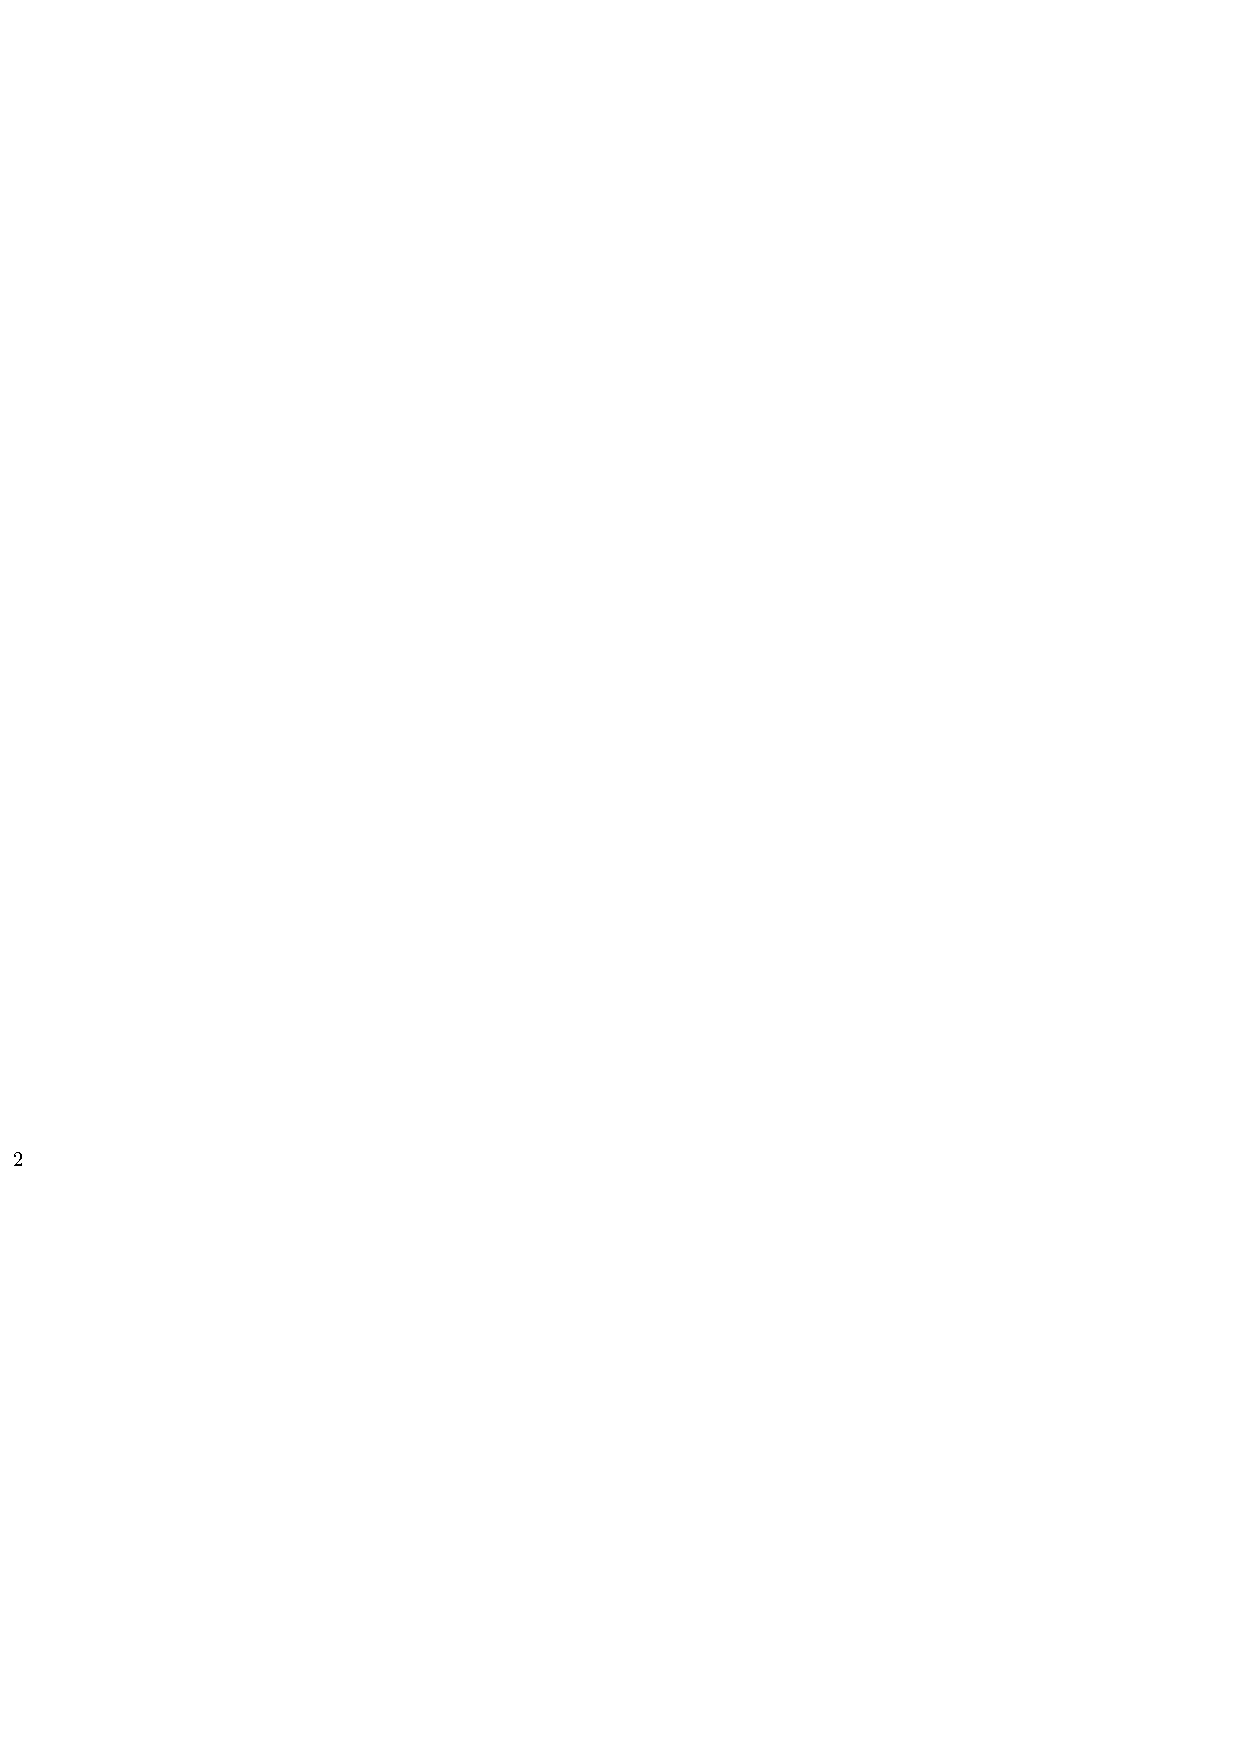
\includegraphics{orient} % omit suffix .eps to supprt PS and PDF
\end{center}
\end{ccTexOnly}
\caption{Orientation of a cell (3-dimensional case)
\label{Triangulation3-fig-orient}}

\begin{ccHtmlOnly}
<CENTER>
<IMG BORDER=0 SRC="./orient.gif" ALIGN=middle ALT="Orientation of a cell
(3-dimensional case)">
</CENTER>
\end{ccHtmlOnly}
\end{figure}
\end{verbatim}

Note above that only the parts that include the two different figure files
are enclosed in the {\tt ccTexOnly} and {\tt ccHtmlOnly} environments.
The {\tt figure}, {\tt caption}, and {\tt label} commands will be processed
for both \LaTeX\  and {\tt latex\_to\_html}.
Note also that the caption and label are placed {\bf above} the HTML picture.
This is done so references to this figure will go to the top of the picture
instead of the bottom (and thus be visible in the browser).
\ccIndexSubitemEnd{manuals}{figures}


% =============================================================================
\section{Indexing\label{sec:indexing}}
\ccIndexSubitemBegin{index}{PDF}
\ccIndexSubitemBegin{manuals}{index}

In order to be truly useful, a manual needs to have an index.  The
{\tt latex\_to\_html} program produces an index for the HTML manual
automatically.  %
\ccIndexSubitem{index}{HTML}\ccIndexSubsubitem{manuals}{HTML}{index}
The style file {\tt cc\_manual\_index.sty}%
\ccIndexMainItem[c]{\tt cc_manual_index.sty} was developed in order to provide
a means for producing an index for the PDF version of the manual.
Though there is also some automatic indexing done by the
{\tt cc\_manual\_index.sty} file in conjunction with {\tt cc\_manual.sty},
this indexing is not sufficient as it can index only things that are
given as arguments to the formatting macros.  When writing your
documentation, you should add other indexing commands in the text in
order to achieve the following goals:
\begin{itemize}
   \item All key words, phrases, topics, and concepts should be indexed.
   \item All \cgal\ \CC\ identifiers described in the manual should be indexed.
   \item There should be listings in the index for any pages on which an
         item is introduced, defined, or described as well as any pages
         where key uses for or instances of these things are described.
   \item There should be sufficient cross referencing to allow users
         to find things starting from many different points.
   \item There should NOT be entries for every mention of every item in the
         manual.
\end{itemize}

You should also take care that the index entries produced by the automatic
indexing are in keeping with these goals, and, when not, use the commands
provided in {\tt cc\_manual\_index.sty} to turn off the automatic indexing.
See the file \ccAnchor{./cc_manual_index.pdf}{{\tt Manual\_tools/doc/cc\_manual\_index.pdf}}
for a description of the commands available and a full description of what
should and should not be indexed.
\ccIndexSubitemEnd{index}{PDF}
\ccIndexSubitemEnd{manuals}{index}



% =============================================================================
\section{Test suite\label{sec:doc_test_suite}}
\ccIndexSubitemBegin{manuals}{test suite}
\ccIndexSubitemBegin{test suite}{for manuals}

With each internal release of the library, a test suite is run on the
manuals to make sure that the documentation submitted makes it through
all the programs and scripts without a problem.  Each package and each
module manual is tested with both \LaTeX\ (and its companion programs
{\tt makeindex} and {\tt bibtex}) and {\tt latex\_to\_html}. The
results of the test suite are currently available at

\hspace*{6mm}\path|http://cgal.geometryfactory.com/CGAL/Members/Manual_test/LAST/|

It is a given, of course, that developers should {\bf test} that their
packages' documentation works with {\bf both} \LaTeX\ and {\tt
  latex\_to\_html} {\bf before} submitting.  The test suite is meant
simply to assure that all the parts fit together nicely and all
references to other parts of the manual get resolved correctly.
Each time you submit a package with modified documentation, you should
check these test results to make sure your documentation did not cause
any problems.
\ccIndexSubitemEnd{manuals}{test suite}
\ccIndexSubitemEnd{test suite}{for manuals}


% =============================================================================
\section{Common problems and solutions\label{sec:common_problems}}

\subsection*{Problem --- Undesired Links in HTML Manual}
\ccIndexSubsubitemBegin{manuals}{HTML}{preventing links}
\ccIndexSubitem{traits class}{naming}

\begin{description}
  \item[{\bf Cause:}] Any occurrence of the name of a class, function,
  etc. that is documented in the reference manual is automatically
  crosslinked to the definition of that entity.

  \item[{\bf Solution:}] Sometimes, the preferred solution is to
  choose a better name for the entity under consideration. For
  example, a traits class for a planar map should be called
  \ccc{Planar_map_traits} rather than \ccc{Traits}. Another
  possibility is to add the command \verb|\ccHtmlNoClassLinks| before
  the \nonlinkedpath|\begin{ccClass}{Traits}| command to globally turn
  off linking of the word \textit{Traits}. To disable links from one
  word only, use the command \verb|\ccHtmlNoLinksFrom|. For example,
  \nonlinkedpath|\ccHtmlNoLinksFrom{Traits}| will not create links for
  this particular occurrence of the word \textit{Traits}.
\end{description}
\ccIndexSubsubitemEnd{manuals}{HTML}{preventing links}

\subsection*{Problem --- Nontransparent backgrounds for HTML figures}
\ccIndexSubsubitemBegin{manuals}{HTML}{figures}

\begin{description}
\item[{\bf Cause:}] The {\tt .gif} file was produced without a transparent
                    background.

\item[{\bf Solution:}] Use either the {\tt giftrans}%
     \index{giftrans script@{\tt giftrans} script}
     program distributed with \LaTeX\ or one of the
     scripts {\tt ps2gif}\index{ps2gif script@{\tt ps2gif} script},
     {\tt ipe2gif}\index{ipe2gif script@{\tt ipe2gif} script}, or
     {\tt latex2gif}\index{latex2gif script@{\tt latex2gif} script}
     that are available from
     \path|http://www.cgal.org/Members/Manual_tools|
     (which use {\tt giftrans} and work for figures with white backgrounds) to
     make the background transparent.
\end{description}
\ccIndexSubsubitemEnd{manuals}{HTML}{figures}

\subsection*{Problem --- Unresolved figure references in HTML}
\ccIndexSubsubitemBegin{manuals}{HTML}{figure references}

%Figure references in the HTML manual appear as ``[ref:fig:xxx]''
%instead of as a link to the figure.

\begin{description}
\item[{\bf Cause:}] This problem is generally caused by the absence of a
     \verb|\label| command inside the HTML figure environment.

\item[{\bf Solution:}]
The easiest way to solve this problem is to put the
\verb|\label| command in the text that is processed by the HTML converter,
as the following example illustrates:

\begin{verbatim}
\begin{figure}[htbp]
\begin{ccTexOnly}
\begin{center}
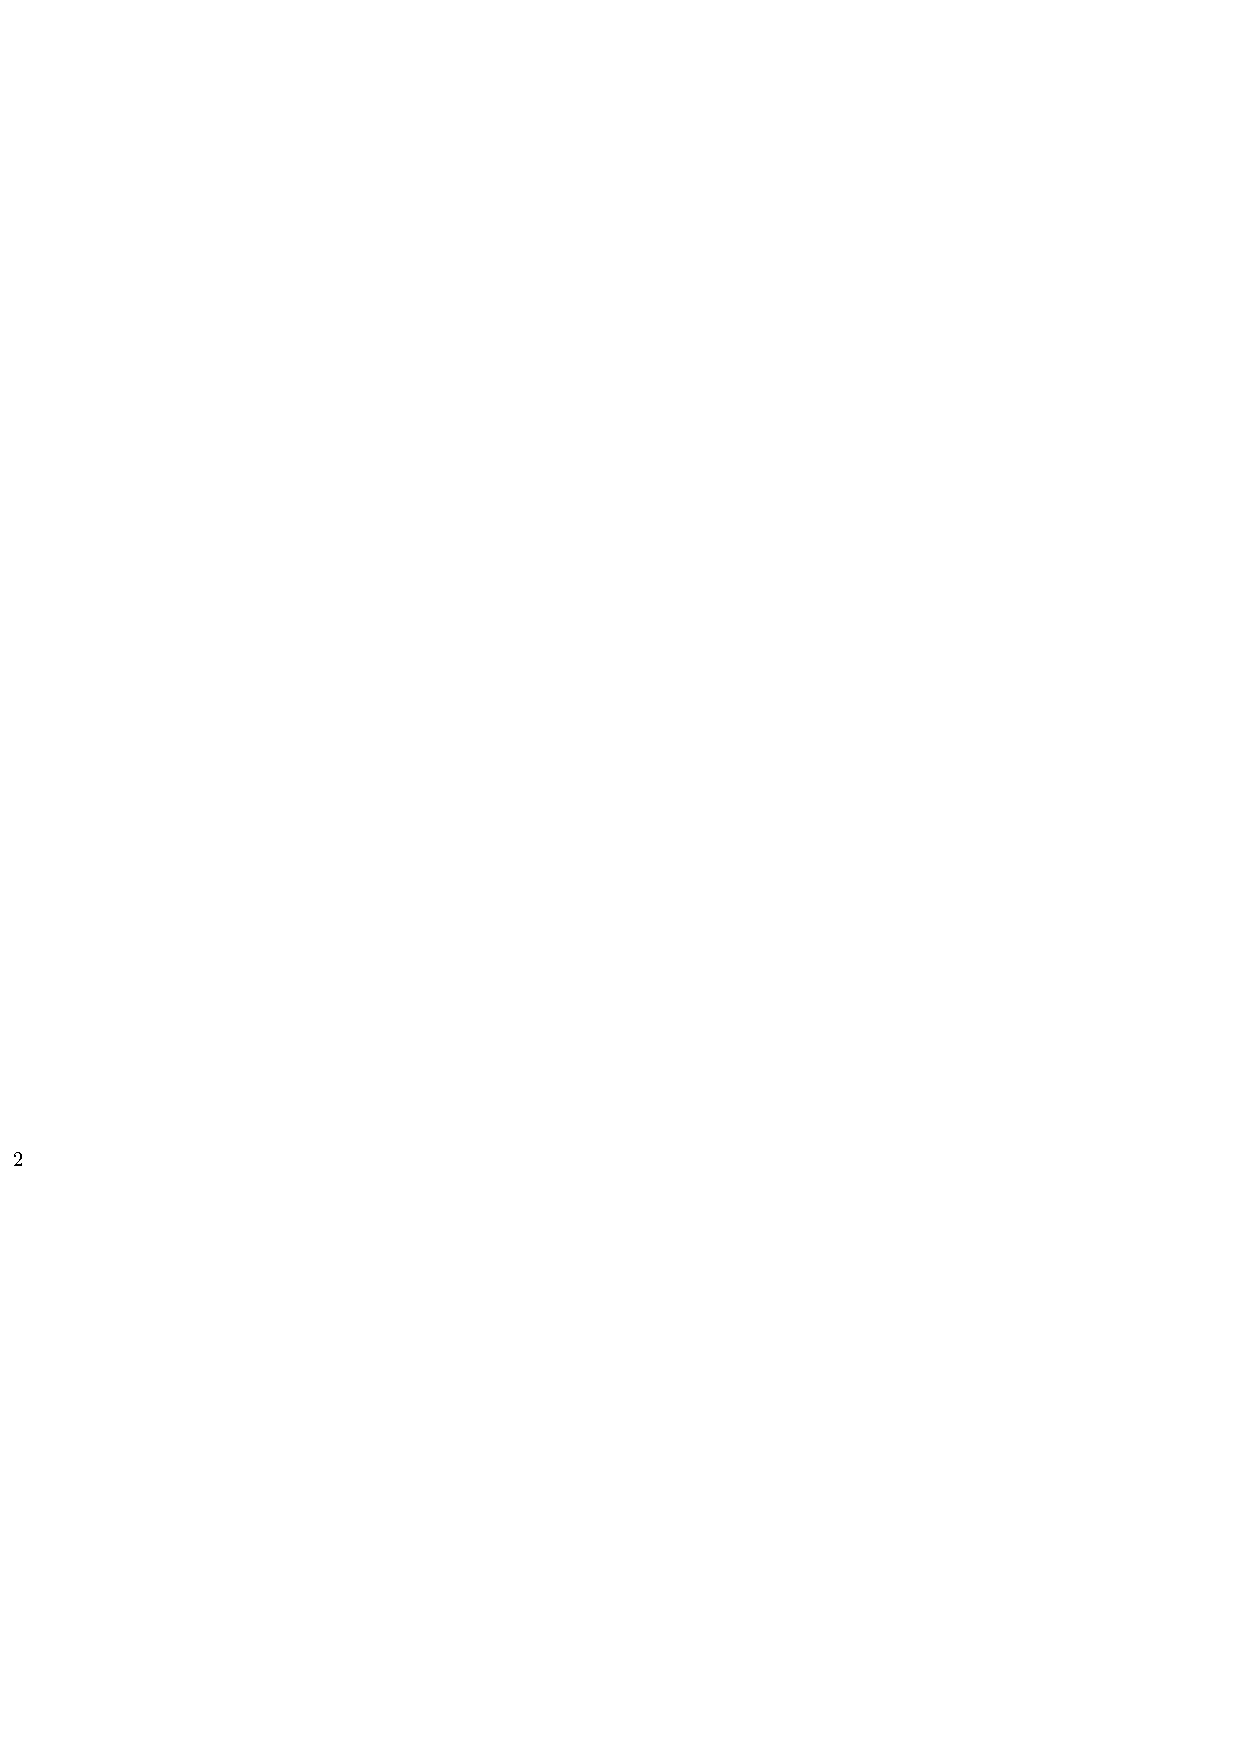
\includegraphics{orient} % omit suffix .eps to supprt PS and PDF
\end{center}
\caption{Orientation of a cell (3-dimensional case)
\label{Triangulation3-fig-orient}}
\end{ccTexOnly}
\lcHtml{\label{Triangulation3-fig-orient}}
\begin{ccHtmlOnly}
<CENTER>
<IMG BORDER=0 SRC="./orient.gif" ALIGN=middle ALT="Orientation of a cell
(3-dimensional case)">
</CENTER>
\end{ccHtmlOnly}
\end{figure}
\end{verbatim}

This will produce a centered figure without a caption in the HTML manual.
References to the label {\tt Triangulation3-fig-orient} will produce a
link that refers to the top of this figure.  If you want the caption with
the HTML figure as well, then simply move the \verb|\end{ccTexOnly}|
command above the \verb|\caption| command and remove the \verb|\lcHtml|
command. See also Section~\ref{sec:doc_figures}.
\ccIndexSubsubitemEnd{manuals}{HTML}{figure references}

\end{description}

\subsection*{Problem --- Raw \LaTeX\ commands in HTML manual}
\index{manuals!HTML!removing raw \LaTeX\ commands|(}
\ccIndexSubsubitemBegin{manuals}{HTML}{unsupported commands}

\begin{description}
\item[{\bf Cause:}] This problem is generally caused by the use of commands
that are not supported by the HTML converter.  See
\ccAnchor{latex_to_html.pdf}{{\tt latex\_to\_html.pdf}} for a list of
these unsupported commands.

\item[{\bf Solution:}] Either remove the offending command altogether or enclose
it in a \verb|\lcTex| command or an {\tt lcTexBlock} environment (which are
both defined in {\tt latex\_converter.sty})\ccIndexMainItem[c]{\tt latex_converter.sty}.
\end{description}
\ccIndexSubsubitemEnd{manuals}{HTML}{unsupported commands}
\index{manuals!HTML!removing raw \LaTeX\ commands|)}

\subsection*{Problem --- Included files cannot be found}
\ccIndexSubsubitemBegin{manuals}{source files}{not found}
\ccIndexSubitemBegin{source files}{documentation}
\ccIndexSubitemBegin{manuals}{environment variables}
\index{input@$\backslash${\tt input}!files not found|(}

\begin{description}
\item[{\bf Cause:}] This problem is generally caused by a wrong relative path
given in the \verb|\input| command (or its derivative) or the absence of a
directory from the appropriate environment variable.

\item[{\bf Solution:}] Paths to source files in other directories must
generally be provided relative to the place where \LaTeX\ and
\texttt{latex\_to\_html} are run, not relative to the place where
the file containing the command is.  When producing the manual,
these programs are run in the \texttt{doc\_tex} directory, so paths
should be relative to this directory.

An exception is for example and demo programs included in the documentation.
\ccIndexSubitem{example programs}{in manuals}.  These should always
be programs that are in the distribution (and thus in the test suite)
and should be included using the command \texttt{ccIncludeExampleCode}.  For
programs you need only specify the path relative to the directory
\texttt{CGAL\_ROOT/examples} or \texttt{CGAL\_ROOT/demo} as the environment
variables \texttt{TEXINPUTS} and \texttt{LATEX\_CONV\_INPUTS} are set so these
directories are searched when the manuals are created with the
\texttt{cgal\_manual} program from Section~\ref{subsec:cgal_manual_program}.
(See
\ccAnchor{./latex_to_html.pdf}{{\tt Manual\_tools/doc/latex\_to\_html.pdf}}
for more details.)
For example, you would use the following command
\begin{verbatim}
   \ccIncludeExampleCode{Polygon/PolygonDemo.cpp}
\end{verbatim}
to include the source file \nonlinkedpath|CGAL_ROOT/demo/Polygon/PolygonDemo.cpp|.
Obviously, you could have problems if you have an example program and a demo
program with the same name in the same package, so try to avoid this.
\end{description}
\index{input@$\backslash${\tt input}!files not found|)}
\ccIndexSubitemEnd{source files}{documentation}
\ccIndexSubitemEnd{manuals}{environment variables}
\ccIndexSubsubitemEnd{manuals}{source files}{not found}


% =============================================================================
\section{Spell checking\label{sec:spell_checker}}

The quality of a manual also depends on the quality of the English.  In order
to help package authors to improve on this aspect, \cgal\ provides a dictionary
of technical terms, to be used together with the \texttt{aspell} spell checking
programs, which helps correcting typos.  Make sure you use it just before
submitting your manual for reviewing by the editorial board, and just before
a public release !

More information on how to use the spell checker can be found in the SVN
repository, under \texttt{/trunk/Manual\_tools/aspell/}.


% =============================================================================
\section{Requirements and recommendations\label{sec:specification_req_and_rec}}

\noindent
Requirements:
\begin{itemize}
   \item Documentation must be written using the {\tt cc\_manual.sty}
         and {\tt cc\_manual\_index.sty} style files.
   \item There must be a {\tt main.tex} file for both the users' manual
         and reference manual parts of the documentation.
   \item Files must be organized according to the directory structure
         outlined in Section~\ref{sec:files_required}.
   \item Indexing commands must be placed in the text to achieve the
         goals listed in Section~\ref{sec:indexing}.
   \item Example programs included in the manual should also be distributed
         in the \texttt{examples} or \texttt{demo} directories and should
         be incorporated in the documentation  using the
         \verb|\ccIncludeExampleCode| command.
\end{itemize}

\noindent
Recommendations:
\begin{itemize}
   \item Documentation of items in the reference manual should use as
         many of the headings listed in Section~\ref{sec:section_headings}
         as appropriate and in the indicated order.
   \item The users' manual should include illustrative examples of a package's
         functionality.
   \item Document each item in the reference manual in its own file.
\end{itemize}

\ccIndexMainItemEnd{manuals}
